\documentclass{beamer}
\usetheme{Warsaw}

\usepackage{graphicx}
\usepackage{tikz}
\usetikzlibrary{arrows.meta}

\title[STARS-$\mathcal{H}$]{\underline{S}oftware for \underline{T}esting
\underline{A}ccuracy, \underline{R}eliability and \underline{S}calability of
$\mathcal{H}$ierarchical computations (STARS-$\mathcal{H}$).}
%\author{A.Mikhalev, H.Ltaief}
\institute{King Abdullah University of Science and Technology}
\date{\today}

\begin{document}

\begin{frame}
\titlepage
\end{frame}

\begin{frame}{Goal of the Project}
\begin{itemize}
\item We want to:\\
Create software for benchmarking performance of operations with hierarchical
matrices of different libraries/tools, measuring results against world-known
algorithms.
\item Supposed results:\\
Classification of software, designed for hierarhical matrices, in different
aspects (not limited to): accuracy, performance, memory footprint and
scalability.
\item Positive side-effect:\\
Relatively easy check for reliability of heavily optimized (device optimized)
algorithms for hierarchical computations.
\end{itemize}
\end{frame}

\begin{frame}{Problem setting}
One of the problems of the project is synthetic generation of hierarchical
matrices with certain properties.
\begin{block}{Desired parameters to be variable}
\begin{itemize}
\item Dimensionality of the problem (influences hierarchical partitioning into
approximately low-rank submatrices).
\item Singular values decay of submatrices (influences ranks of submatrices),
\item Common row/column basises of submatrices (influences singular values
decay of unions of submatrices, i.e. making $\mathcal{H}^2$-matrices
suitable or unsuitable),
\end{itemize}
\end{block}
\begin{alertblock}{}
Synthetic generation of matrices will make it possible to test future
algorithms for reliability before applying for real problems.
\end{alertblock}
\end{frame}

\begin{frame}{Synthetic matrix generation}
\begin{enumerate}
\item \textit{Analitycal}: by a function for each element of a matrix.\\
\textcolor{green}{+}: comes from real problems.\\ \textcolor{red}{--}: need to
build approximation in hierarchical format.
\item \textit{Algebraical}: by a given approximation in hierarchical
format.\\ \textcolor{green}{+}: may come from real problems.\\
\textcolor{red}{--}: it is hard to test such a matrices with different
hierarchical formats (because of conversion to dense).
\item \textit{Semi-analitycal}: by a specially selected per-element
functions.\\ \textcolor{green}{+}: approximation in hierarchical formats is
known apriori.\\ \textcolor{red}{--}: Does not deal with real problems, but can
mimic them by means of decay of singular values of submatrices.
\end{enumerate}
\begin{alertblock}{}
Obviously, synthetic $\mathcal{H}$-matrices should be generated in a
semi-analitycal way to expose known apriori $\mathcal{H}$-structure.
\end{alertblock}
\end{frame}

\begin{frame}{First idea}
Desired matrix may look like $A = UV^T+D,$ where $D$ is a diagonal and $U$ and
$V$ have corresponding sizes. Then, function of matrix generation may look like
$A_{i,j} = \sum_{k=1}^{R} U_{i,k}V_{j,k}$.
\begin{center}
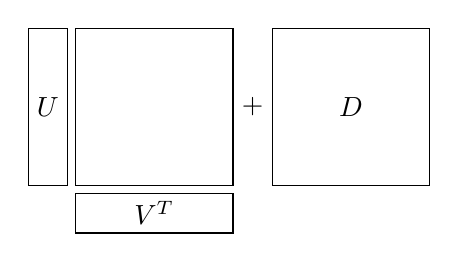
\begin{tikzpicture}
\draw (0,0) rectangle +(2,2);
\draw (-0.6,0) rectangle +(0.5,2);
\node at (-0.35,1) {$U$};
\draw (0,-0.6) rectangle +(2,0.5);
\node at (1,-0.35) {$V^T$};
\node at (2.25,1) {$+$};
\draw (2.5,0) rectangle +(2,2);
\node at (3.5,1) {$D$};
\end{tikzpicture}
\end{center}
\begin{alertblock}{This leads to}
semi-separable, $\mathcal{H}$ and flat $\mathcal{H}$ (all blocks are of the
same size) matrices. Rank of any off-diagonal block equals to minimum of ranks
of $U$ and $V$.
\end{alertblock}
\end{frame}

\begin{frame}{Flat $\mathcal{H}$ matrix}
\begin{center}
\begin{block}{Assumption on structure}
$A_{i,j}=U_iS_{i,j}V_j^T$, size of every block $A_{i,j}$ is the same. $U_i$ and
$V_j$ are orthogonal, $S_{i,j}$ is diagonal.
\end{block}
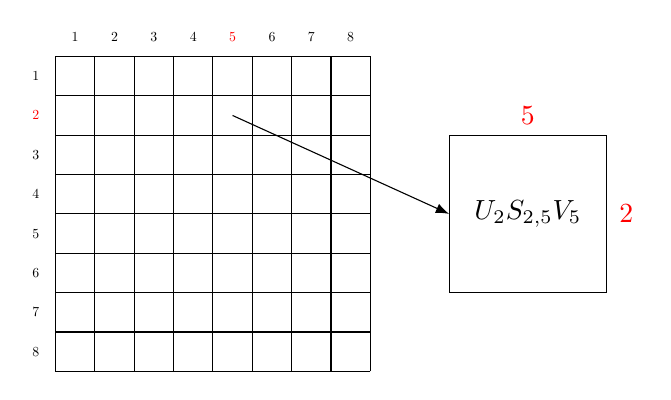
\begin{tikzpicture}
\draw[step=0.5] (0,0) grid +(4,4);
\draw[-Latex] (2.25,3.25) -- (5,2);
\draw (5,1) rectangle +(2,2);
\node at (-0.25,0.25) [scale=0.5]{8};
\node at (-0.25,0.75) [scale=0.5]{7};
\node at (-0.25,1.25) [scale=0.5]{6};
\node at (-0.25,1.75) [scale=0.5]{5};
\node at (-0.25,2.25) [scale=0.5]{4};
\node at (-0.25,2.75) [scale=0.5]{3};
\node at (-0.25,3.25) [scale=0.5]{\color{red}2};
\node at (-0.25,3.75) [scale=0.5]{1};
\node at (0.25,4.25) [scale=0.5]{1};
\node at (0.75,4.25) [scale=0.5]{2};
\node at (1.25,4.25) [scale=0.5]{3};
\node at (1.75,4.25) [scale=0.5]{4};
\node at (2.25,4.25) [scale=0.5]{\color{red}5};
\node at (2.75,4.25) [scale=0.5]{6};
\node at (3.25,4.25) [scale=0.5]{7};
\node at (3.75,4.25) [scale=0.5]{8};
\node at (6,2) {$U_2 S_{2,5} V_5$};
\node at (6,3.25) {\color{red}5};
\node at (7.25,2) {\color{red}2};
\end{tikzpicture}
\end{center}
\end{frame}

\begin{frame}{Flat $\mathcal{H}$ matrix}
\begin{block}{Assumption on structure}
Each $S_{i,j}$ contains nonegative descending values.
\end{block}
$$\begin{bmatrix} A_{1,2} & A_{1,3} \end{bmatrix} = U_1 \begin{bmatrix}
S_{1,2} V_2 & S_{1,3} V_3 \end{bmatrix}.$$
Low-rankness of $U_1$ leads to low-rankness of entire block row, based on first
block of rows.
\begin{alertblock}{}
Approximation of each block by a low-rank matrix leads to approximation of
entire block rows/columns by a low-rank matrix (with the same rank, as per
block). Addition of noise or rotation of $U_1$ for each different $A_{1,j}$ is
required.
\end{alertblock}
\end{frame}

\begin{frame}{Generation with help of Fourier matrices}
\begin{block}{Assumption}
Let $U_i=V_j=F$, where $F$ is a Fourier matrix of corresponding size.
\end{block}
Then, element on row $k$ on column $l$ of a matrix $A$ can be generated by a
simple function:
$$A_{k,l} = \sum_{r=1}^R F_{k,r} S_{i,j,r} F_{l,r},$$
where $R$ is a size of block, $F_{k,r}$ is an lement of Fourier matrix on
$k$-th row on $r$-th column, $i$ is a number of block row, containing row $k$,
$j$ is a number of block column, containing column $l$, $S_{i,j,r}$ is $r$-th
value of diagonal matrix $S_{i,j}$ and $F_{l,r}$ is a corresponding element of
Fourier matrix of size $R$.
\end{frame}

\begin{frame}{To-Do list}
\begin{itemize}
\item Add noise to $S_{i,j}$ (drawback: requires storage of each $S_{i,j}$,
which is $O(N^2)$, where $N$ is a number of rows of the matrix),
\item Try to mimic nonidentical singular rows/columns of submatrices by
applying rotations (one rotation matrix for each block of rows/columns).
\item Try other assumptions?
\end{itemize}
\end{frame}

\end{document}
